\documentclass{standalone}
\usepackage{graphicx}	
\usepackage{amssymb, amsmath, amsthm}
\usepackage{color}

\usepackage{tikz}
\usetikzlibrary{intersections, backgrounds, math}

\definecolor{mid}{RGB}{220, 188, 188}
\definecolor{mid}{RGB}{185, 124, 124}
\definecolor{dark}{RGB}{143, 39, 39}
\definecolor{highmid}{RGB}{180, 31, 180}
\definecolor{gray10}{gray}{0.1}
\definecolor{gray20}{gray}{0.2}
\definecolor{gray30}{gray}{0.3}
\definecolor{gray40}{gray}{0.4}
\definecolor{gray60}{gray}{0.6}
\definecolor{gray70}{gray}{0.7}
\definecolor{gray80}{gray}{0.8}
\definecolor{gray90}{gray}{0.9}
\definecolor{gray95}{gray}{0.95}

\begin{document}

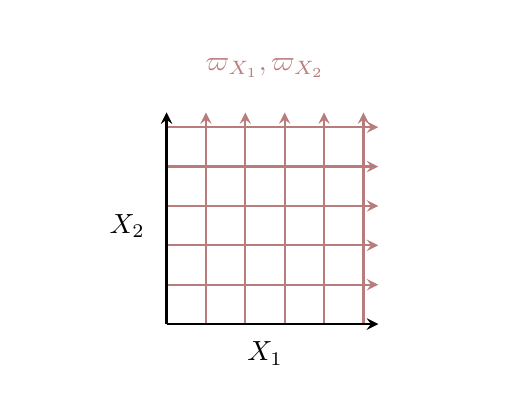
\begin{tikzpicture}[scale=0.25, thick]
  
  \pgfmathsetmacro{\dx}{0}
  
  \draw[white] (-12 + \dx, -8) rectangle (12 + \dx, 10);
  
  \draw[black, line width=0.3, fill=white] (-5, -5) -- (5, -5) -- (5, 5) -- (-5, 5) -- (-5, -5);
  
  \foreach \x in {0, 1, ..., 5} {
    \draw[mid, ->, >=stealth] (2 * \x - 5 + \dx, -5) -- (2 * \x - 5 + \dx, 5.75);
  }

  \foreach \y in {0, 1, ..., 5} {
    \draw[mid, ->, >=stealth] (-5 + \dx, 2 * \y - 5) -- (5.75 + \dx, 2 * \y - 5);
  }
  
  \draw[black, ->, >=stealth] (-5, -5) -- (5.75, -5);
  \node[black] at (0, -6.5) {$X_{1}$};

  \draw[black, ->, >=stealth] (-5, -5) -- (-5, 5.75);
  \node[black] at (-7, 0) {$X_{2}$};
  
  \node[mid] at (0, 8) {$\varpi_{X_{1}}, \varpi_{X_{2}}$};
  
\end{tikzpicture}

\end{document}  